% \documentclass{article}

\documentclass{article}
%% \documentclass[twocolumn]{article}

\renewcommand{\familydefault}{\sfdefault} % Standardfont ändern auf Sans Serif (bny)

\usepackage[utf8x]{inputenc}
\usepackage[german]{babel} % Sprache umschalten /hat funktioniert bis auf Authors, bny 13.04.2016
\usepackage{tcolorbox}
\usepackage{xcolor}
\definecolor{chamois}{rgb}{1,.984314,.956863}  % RGB 255 247 231
\pagecolor{chamois}
\usepackage{geometry}
\geometry{verbose,a4paper,tmargin=10mm,bmargin=10mm,lmargin=10mm,rmargin=10mm}

\usepackage{multicol} % 20.04.2017 hinzugefügt, bny

%%% \usepackage{tikz}
%%% % \pagecolor{olive!50!yellow!50!white}

\tcbuselibrary{skins}

\colorlet{xlightblue}{blue!5}

\newtcolorbox{beamerlikethm}[1]{
  title=#1,
  beamer,
  % colback=xlightblue,
  colframe=red!50,
  fonttitle=\bfseries,
  left=1mm,
  right=1mm,
  top=1mm,
  bottom=1mm,
  middle=1mm
}


\begin{document}
\pagestyle{empty}

%%% \begin{tikzpicture}[remember picture, overlay]
%%% \shade[left color=red!50,
%%% right color=green!50
%%% ] (current page.north west) rectangle (current page.south east);
%%% \end{tikzpicture}

\centering{{\huge Dokumentenablage}}

\vspace{\baselineskip}

%%%%%%

% \begin{beamerlikethm}{Eine Sitzungseinladung bearbeiten}
% \begin{itemize}
%   \item[$\Longrightarrow$] Wählen Sie die gewünschte Sitzung aus. Klicken Sie auf den Titel. Die Optionen öffnen sich.
%  \item[$\Longrightarrow$] Klicken Sie auf das Bearbeitungssymbol. Nun können Sie die gewünschten Änderungen vornehmen.
%   \item[$\Longrightarrow$] Schliessend Sie den Vorgang erneut mit Klick auf 'Übernahme' ab.
% \end{itemize}
% \end{beamerlikethm}


%%%% Box 1+2 in zwei Spalten

\begin{multicols}{2}

\begin{tcolorbox}[colback=blue!5,colframe=blue!40!black,title=Dokumente hochladen]
\begin{itemize}
  \item[$\Longrightarrow$] Klicken Sie auf das 
\includegraphics[height=10pt]{Icons/Plussymbol.jpg}, die Eingabemaske öffnet sich.
  \item[$\Longrightarrow$] Ziehen Sie das gewünschte File in das Feld 'Datei' oder geben Sie einen Link in das Feld 'Adresse' ein.
  \item[$\Longrightarrow$] Füllen Sie die anderen Felder aus.
  \item[$\Longrightarrow$] Bevor Sie das Dokument mittels 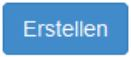
\includegraphics[height=12pt]{Icons/B_Erstellen.jpg} speichern können, müssen Sie noch mindestens eine Zugriffsberechtigung definieren. 
	\item[$\Longrightarrow$] Dazu klicken Sie auf 
\includegraphics[height=10pt]{Icons/Pluszeichen.jpg} und fügen (in der Regel) ihren Namen und die gewünschten Berechtigungen hinzu.
	\item[$\Longrightarrow$] Schliessen Sie den Vorgang nun mit 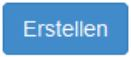
\includegraphics[height=12pt]{Icons/B_Erstellen.jpg} ab.
\end{itemize}
\end{tcolorbox}


\begin{tcolorbox}[colback=blue!5,colframe=blue!40!black,title=Dokumente mit Google-Maps verknüpfen]
\begin{itemize}
  \item[$\Longrightarrow$] Wählen Sie das gewünschte Dokument aus und klicken Sie auf  
\includegraphics[height=10pt]{Icons/bearbeiten.jpg}.
  \item[$\Longrightarrow$] Klicken Sie oben rechts im Bearbeitungsfenster auf 'Karte anzeigen / verstecken'. Google-Maps wird nun angezeigt.
  \item[$\Longrightarrow$] Durch Klick auf die linke Maustaste können Sie den Kartenauschnitt verschieben; mittels einem Scroll-Rad können Sie die Karte vergrössern oder verkleinern.
  \item[$\Longrightarrow$] Haben Sie den gewünschten geographischen Ort gefunden, machen Sie dort mit der Maus einen Doppelklick. Es wird eine Nadel gesetzt: 
\includegraphics[height=10pt]{Icons/vNadel.jpg}.
	\item[$\Longrightarrow$] Sie können die 
\includegraphics[height=10pt]{Icons/vNadel.jpg} jederzeit wieder verschieben oder mittels Rechtsklick löschen.
\end{itemize}
\end{tcolorbox}


\end{multicols}

%%%% Box 3+4 in zwei Spalten

\begin{multicols}{2}

\begin{tcolorbox}[colback=blue!5,colframe=blue!40!black,title=Bearbeiten von Dokumenten]
\begin{itemize}
  \item[$\Longrightarrow$] Klicken Sie in der Dokumentenübersicht auf den Titel des gewünschten Dokuments. Es öffnen sich die Optionen.
  \item[$\Longrightarrow$] Klicken Sie auf 
\includegraphics[height=12pt]{Icons/Auschecken.jpg}. Das Dokument wird ausgeckeckt und im Word geöffnet.
  \item[$\Longrightarrow$] Bearbeiten Sie das Dokument und klicken Sie fürs Speichern 
\includegraphics[height=12pt]{Icons/Sync2013.jpg} oder 
\includegraphics[height=12pt]{Icons/Sync2016.jpg} oben links im Word. Das Dokument wird gleich wieder in CUBE gespeichert.
  \item[$\Longrightarrow$] Sie können die Arbeit unterbrechen und zu einem anderen Zeitpunkt mit Klick auf 
\includegraphics[height=12pt]{Icons/Wolke_blauklein.jpg} das Dokument weiterbearbeiten. Beachten Sie, dass in dieser Zeit niemand sonst am Dokument arbeiten kann.
	\item[$\Longrightarrow$] Sind Sie mit der Überarbeitung fertig, speichern Sie das Dokument und klicken auf  
\includegraphics[height=10pt]{Icons/Einchecken.jpg}. Das Dokument wird eingecheckt und steht für die anderen Personen wieder zur Verfügung.
\end{itemize}
\end{tcolorbox}


\begin{tcolorbox}[colback=blue!5,colframe=blue!40!black,title=Finden von Dokumenten]
\begin{itemize}
  \item[$\Longrightarrow$] In der Dokumentenübersicht können Sie im Feld 'Volltextsuche' den gewünschten Suchbegriff eingeben.
  \item[$\Longrightarrow$] Sie können in sämtlichen Spalten ebenfalls Suchbegriffe eingeben und nach diesen Eingaben filtern.
  \item[$\Longrightarrow$] Haben Sie Suchbegriffe eingegeben, klicken Sie auf  
\includegraphics[height=9pt]{Icons/Lupe_s.jpg} oder drücken die Entertaste.
  \item[$\Longrightarrow$] Die Anzeige wird gefiltert. Löschen Sie die überflüssigen Suchworte wieder und klicken Sie erneut auf  
\includegraphics[height=9pt]{Icons/Lupe_s.jpg}.
	\item[$\Longrightarrow$] Sämtlich angezeigte Dokumente können Sie mit Klick auf die entsprechende Spaltenüberschrift von A-Z oder Z-A sortieren.
	\item[$\Longrightarrow$] Bei den Spalten mit 
\includegraphics[height=9pt]{Icons/Pfeil_rechts.jpg}-Symbol können Sie die Suche mit 'und/oder' erweitern und so ein gezielteres Suchresultat erreichen.
\end{itemize}
\end{tcolorbox}


\end{multicols}


%%% HINWEISE %%%
%%% Hinweise in 1er Spalte

\begin{beamerlikethm}{Hinweise}
\begin{itemize}
  \item[$\Longrightarrow$] Ein Dokument kann nur durch ein anderes ersetzt werden. Beim Versuch mehrere Dokumente in das Uploadfenster zu ziehen, erscheint eine Fehlermeldung.
 \item[$\Longrightarrow$] Werden bei einem Dokument nur die Metadaten geändert, wird keine neue Dokumentenversion gespeichert.
 \item[$\Longrightarrow$] Ein von Ihnen ausgechecktes Dokument erscheint automatisch in ihrer persönlichen Projektübersicht. Sie können das Dokument direkt zur weiteren Bearbeitung öffnen oder wieder einchecken.
 \item[$\Longrightarrow$] Das online-Bearbeiten von Dokumenten ist mit den gängigen MS Office Programmen durchführbar. Dokumente in anderen Formaten (z.B. PDF oder CAD-Pläne) können
zwar auch ausgecheckt werden, eine online-Bearbeitung ist aber nicht möglich.
 \item[$\Longrightarrow$] Ein ausgechecktes Dokument kann durch weitere Benutzer nicht bearbeitet werden und ist gesperrt. Es erscheint in den Optionen ein 
\includegraphics[height=10pt]{Icons/Warnung_rot.jpg}.
\end{itemize}
\end{beamerlikethm}


  %%%%%%
	% Spalte 2
	%%%%%%
	
	% Reserve
	
% 	\begin{tcolorbox}[colback=blue!5,colframe=blue!40!black,title=Protokoll bearbeiten]
% \begin{itemize}
%   \item[$\Longrightarrow$] Kehren Sie zur Übersicht zurück
%   \item[$\Longrightarrow$] Wählen Sie die gewünschte Sitzung aus und klicken Sie auf den blauen Titel. Die Optionen öffnen sich
%   \item[$\Longrightarrow$] Klicken Sie auf das Protokollsymbol. Das Sitzungsprotokoll wird geöffnet.
%   \item[$\Longrightarrow$] Sie können das erstellte PDF per Email oder auch per Post versenden.
% \end{itemize}
% \end{tcolorbox}

%%%%%%%%%%%%%%%%%%%%%%%%%%%	
%%%%%%% Neue Seite %%%%%%%%
%%%%%%%%%%%%%%%%%%%%%%%%%%%


\pagebreak

\centering{{\huge Sitzungswesen}}

\vspace{\baselineskip}


%%%% Box 1+2 in zwei Spalten

\begin{multicols}{2}

\begin{tcolorbox}[colback=blue!5,colframe=blue!40!black,title=Zu einer neuen Sitzung einladen]
\begin{itemize}
  \item[$\Longrightarrow$] Klick auf 
\includegraphics[height=10pt]{Icons/Plussymbol.jpg} und benötigte Felder ausfüllen.
  \item[$\Longrightarrow$] Wahlweise eine vordefinierte Teilnehmerliste (im Dropdownmenü Liste auswählen) und 'übernehmen' klicken oder einzelne Personen mit 
\includegraphics[height=12pt]{Icons/Pluszeichen.jpg} hinzufügen.
  \item[$\Longrightarrow$] Sind Eingaben getätigt, Klick auf 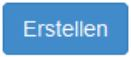
\includegraphics[height=12pt]{Icons/B_Erstellen.jpg}. 
	\item[$\Longrightarrow$] Details für die Sitzungseinladung hinzufügen: Vordefinierte Traktandenliste auswählen und 'übernehmen' klicken.
  \item[$\Longrightarrow$] oder mit Klick auf 
\includegraphics[height=12pt]{Icons/Pluszeichen.jpg}  einzelne Traktanden eingeben.
  \item[$\Longrightarrow$] Unter 'Beilagen' Dokumente oder Bilder für die Sitzung hochladen.						
	\item[$\Longrightarrow$] Vorgang mit 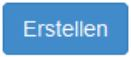
\includegraphics[height=12pt]{Icons/B_Erstellen.jpg} abschliessen.
\end{itemize}
\end{tcolorbox}


%% bishierher


\begin{tcolorbox}[colback=blue!5,colframe=blue!40!black,title=Eine Einladung bearbeiten / versenden]
\begin{itemize}
  \item[$\Longrightarrow$] Geben Sie die Sitzungseinladung mit Setzen des Häkchens 
\includegraphics[height=12pt]{Icons/sbox_ok.jpg} (oben links) frei. Diese erscheint nun in Ihrer persönlicher Übersicht.
  \item[$\Longrightarrow$] Wuzrden alle benötigten Eingaben gemacht, können Sie mit dem 
\includegraphics[height=12pt]{Icons/Briefsymbol.jpg} ein PDF der Sitzungseinladung generieren und anschliessend per Mail oder in Papierform versenden.
  \item[$\Longrightarrow$] Mit Klick auf das 
\includegraphics[height=12pt]{Icons/Listensymbol.jpg}, können Sie das Protokoll bearbeiten. In diesem Modus werden die Traktanden bearbeitet, daraus Pendenzen oder Entschlüsse gemacht.		
\end{itemize}
\end{tcolorbox}


\end{multicols}

%%%% Box 3+4 in zwei Spalten

\begin{multicols}{2}

\begin{tcolorbox}[colback=blue!5,colframe=blue!40!black,title=Das Protokoll führen]
\begin{itemize}
  \item[$\Longrightarrow$] Befinden Sie sich im Protokollmodus (erreichbar durch das 
\includegraphics[height=10pt]{Icons/Listensymbol.jpg}-Symbol), können Sie die Traktanden bearbeiten, resp. die nötigen Einträge vornehmen.
	\item[$\Longrightarrow$] Mit Klick rechts des Traktandums auf 
\includegraphics[height=10pt]{Icons/Blattsymbol.jpg} werden die Optionen geöffnet:
  \item[$\Longrightarrow$] Mit den Funktionen 
\includegraphics[height=10pt]{Icons/Gutzeichen_Rahmen.jpg} oder 
\includegraphics[height=10pt]{Icons/Pfeil_Gutzeichen.jpg} können Sie aus einem Traktandum einen Entscheid erstellen oder das Traktandum in einen Entscheid umwandeln.
	  \item[$\Longrightarrow$] Mit den Funktionen 
\includegraphics[height=10pt]{Icons/Pfeil_aus_Box.jpg} oder 
\includegraphics[height=10pt]{Icons/Pfeil_Pfeil_aus_Box.jpg} können Sie aus einem Traktandum eine Pendenz erstellen oder das Traktandum in eine Pendenz umwandeln.
  \item[$\Longrightarrow$] Klicken Sie auf das 
\includegraphics[height=10pt]{Icons/Blattsymbol.jpg}, um aus dem Protokoll ein PDF zu erstellen. Dieses können Sie im Anschluss an die Teilnehmer versenden und archivieren.
	\item[$\Longrightarrow$] Im Protokollmodus haben Sie zudem die Möglichekti, ein separates PDF-Protokoll hochzuladen. Klicken Sie dazu bei 'Protokoll hochladen' auf 'Durchsuchen' und wählen Sie das gewüschte Protokoll aus.
	\item[$\Longrightarrow$] Wurde ein Protokoll Archiviert, lässt es sich nicht mehr verändern und auch nicht mehr löschen.
\end{itemize}
\end{tcolorbox}


\begin{tcolorbox}[colback=blue!5,colframe=blue!40!black,title=Pendenz- und Entscheid-Listen]
\begin{itemize}
  \item[$\Longrightarrow$] Sie haben die Möglichkeit direkt aus den Traktanden (Im Protokollmodus) Pendenzen oder Entscheide zu erstellen (Siehe nächste Box).
  \item[$\Longrightarrow$] Sie können zudem ohne Protokoll neue Pendenzen und Entscheide erstellen: 
  \item[$\Longrightarrow$] Wählen Sie im Hauptmenü unter 'Sitzungswesen' den Punkt 'Pendenzen' oder 'Entscheide' an. Sie können jeweils mit 
\includegraphics[height=9pt]{Icons/Plussymbol.jpg} eine neue Pendenz oder ein neuer Entscheid Hinzufügen.
  \item[$\Longrightarrow$] Füllen Sie alle gewünschten Felder aus und achten Sie auf die Pflichtfelder (*). 
	\item[$\Longrightarrow$] In der Übersicht der Pendenzen und Entscheide können Sie mit der Volltextsuche oder der Suche nach bestimmten Angaben wie (ID, Titel, Beschreibung) nach Pendenzen und Entscheiden suchen.
	\item[$\Longrightarrow$] Pendenzen werden terminiert. In der Übersicht zeigt ein Ampelsystem, ob eine Pendenz überfällig (
\includegraphics[height=9pt]{Icons/PunktRot.jpg}), die Fälligkeit bald erreicht ist (
\includegraphics[height=9pt]{Icons/PunktGelb.jpg}) oder der Endtermin  'in weiter Ferne' liegt (
\includegraphics[height=9pt]{Icons/PunktGruen.jpg}).
\end{itemize}
\end{tcolorbox}


\end{multicols}


%%% HINWEISE %%%
%%% Hinweise in 1er Spalte

\begin{beamerlikethm}{Hinweise/Tipps}
\begin{itemize}
  \item[$\Longrightarrow$] Anstelle eines Klicks auf 'Durchsuchen' beim Hochladen einer Beilage  können Sie die gewünschte Datei mit der Maus auf das Feld 'Durchsuchen' ziehen und loslassen.
  \item[$\Longrightarrow$] Im Protokollmodus haben Sie die Möglichkeit mittels den 
\includegraphics[height=9pt]{Icons/Pfeil-links-rechts.jpg}-Symbolen die Trakdanden in 1, 1.1 oder ohne Nummer zu gliedern.
	\item[$\Longrightarrow$] Für  Protokollprüfung durch Teilnehmer, klick in das Traktandumfenster und mit 
\includegraphics[height=9pt]{Icons/UeberarbModus.jpg} Überarbeitungsmodus einschalten. Alle Änderungen werden nun protokolliert.
\end{itemize}
\end{beamerlikethm}

  %%%%%%
	% Spalte 2
	%%%%%%
	
	% Reserve
	
% 	\begin{tcolorbox}[colback=blue!5,colframe=blue!40!black,title=Protokoll bearbeiten]
% \begin{itemize}
%   \item[$\Longrightarrow$] Kehren Sie zur Übersicht zurück
%   \item[$\Longrightarrow$] Wählen Sie die gewünschte Sitzung aus und klicken Sie auf den blauen Titel. Die Optionen öffnen sich
%   \item[$\Longrightarrow$] Klicken Sie auf das Protokollsymbol. Das Sitzungsprotokoll wird geöffnet.
%   \item[$\Longrightarrow$] Sie können das erstellte PDF per Email oder auch per Post versenden.
% \end{itemize}
% \end{tcolorbox}


\pagebreak

\centering{{\huge Beschaffungswesen}}

\vspace{\baselineskip}

%% bishierher

%%%% Box 1+2 in zwei Spalten

\begin{multicols}{2}

\begin{tcolorbox}[colback=blue!5,colframe=blue!40!black,title=(1) Neue Beschaffung initialisieren]
\begin{itemize}
  \item[$\Longrightarrow$] Vorbereitung: Erstellen Sie sämtliche Dokumente zur Offertenanfrage ausserhalb von CUBE PA.
  \item[$\Longrightarrow$] Klick auf 
\includegraphics[height=10pt]{Icons/Plussymbol.jpg} und füllen Sie alle benötigten Felder aus.
  \item[$\Longrightarrow$] Beachten Sie die Pflichtfelder. Der Status ist 'Erstellung Ausschreibung'
  \item[$\Longrightarrow$] Klicken Sie auf 'Übernehmen' oben in der Mitte des Bildes oder auf 'Erstellen' unterhalb der Felder.
	\item[$\Longrightarrow$] Erst jetzt ist es Möglich die Ausschreibungsunterlagen hochzuladen.
  \item[$\Longrightarrow$] Schliessen Sie diesen Vorgang ebenfalls mit 'Übernehmen' ab. Die Ausschreibung wurde erstellt.
	\item[$\Longrightarrow$] Dokumentenprüfung und Fertigstellung durch Kunde.
\end{itemize}
\end{tcolorbox}


%% bishierher


\begin{tcolorbox}[colback=blue!5,colframe=blue!40!black,title=(2) Offertanfrage versenden]
\begin{itemize}
  \item[$\Longrightarrow$] Gewünschte Beschaffung öffnen. Spätestens jetzt 'Eingeladene' hinzufügen und alle nötigen Anpassungen vornehmen.
	\item[$\Longrightarrow$] Klick auf 'Senden' 
\includegraphics[height=12pt]{Icons/Versandsymbol.jpg}. Auswahl Versand per Email oder Brief.
  \item[$\Longrightarrow$] Email: Emailvorlage mit Link wird erstellt. Brief: Briefvorlage mit Einladungstext wird erstellt (pdf).
  \item[$\Longrightarrow$] Status ändern auf 'Ausschreibung versendet'. Vorgang abschliessen mit 'Übernehmen'.
\end{itemize}
\end{tcolorbox}


\end{multicols}

%%%% Box 3+4 in zwei Spalten

\begin{multicols}{2}

\begin{tcolorbox}[colback=blue!5,colframe=blue!40!black,title=(3) Offerte(n) entgegennehmen und prüfen]
\begin{itemize}
  \item[$\Longrightarrow$] Eingehende Offerten in CUBE erfassen
	\item[$\Longrightarrow$] Mit Klick rechts des Traktandums auf 
\includegraphics[height=10pt]{Icons/Blattsymbol.jpg} werden die Optionen geöffnet:
  \item[$\Longrightarrow$] Mit den Funktionen 
\includegraphics[height=10pt]{Icons/Gutzeichen_Rahmen.jpg} oden Sie aus einem Traktandunen Entscheid umwandeln.
	\item[$\Longrightarrow$] Mit den Funktionen 
\includegraphics[height=10pt]{Icons/Pfeil_aus_Box.jpg} nen Sie aus einem Traktandum eine Pendenz erstellen oder das Traktandum in eine Pendenz umwandeln.
  \item[$\Longrightarrow$] Klicken Sie auf das 
\includegraphics[height=10pt]{Icons/Blattsymbol.jpg}, um aAnschluss an die Teilnehmer versenden und archivieren.
	\item[$\Longrightarrow$] Im Protokollmodus haben Sie zudem die Möglichekti, ein separauchen' und wählen Sie das gewüschte Protokoll aus.
	\item[$\Longrightarrow$] Wurde ein Protokoll Archiviert, lässt es sich nicht mehr verändern und auch nicht mehr löschen.
\end{itemize}
\end{tcolorbox}


\begin{tcolorbox}[colback=blue!5,colframe=blue!40!black,title=Pendenz- und Entscheid-Listen]
\begin{itemize}
  \item[$\Longrightarrow$] Sie haben die Möglichkeit direkt aus den Traktanden (Im Protokollmodus) Pendenzen oder Entscheide zu erstellen (Siehe nächste Box).
  \item[$\Longrightarrow$] Sie können zudem ohne Protokoll neue Pendenzen und Entscheide erstellen: 
  \item[$\Longrightarrow$] Wählen Sie im Hauptmenü unter 'Sitzungswesen' den Punkt 'Pendenzen' oder 'Entscheide' an. Sie können jeweils mit 
\includegraphics[height=9pt]{Icons/Plussymbol.jpg} eine neue Pendenz oder ein neuer Entscheid Hinzufügen.
  \item[$\Longrightarrow$] Füllen Sie alle gewünschten Felder aus und achten Sie auf die Pflichtfelder (*). 
	\item[$\Longrightarrow$] In der Übersicht der Pendenzen und Entscheide können Sie mit der Volltextsuche oder der Suche nach bestimmten Angaben wie (ID, Titel, Beschreibung) nach Pendenzen und Entscheiden suchen.
	\item[$\Longrightarrow$] Pendenzen werden terminiert. In der Übersicht zeigt ein Ampelsystem, ob eine Pendenz überfällig (
\includegraphics[height=9pt]{Icons/PunktRot.jpg}), die Fälligkeit bald erreicht ist (
\includegraphics[height=9pt]{Icons/PunktGelb.jpg}) oder der Endtermin  'in weiter Ferne' liegt (
\includegraphics[height=9pt]{Icons/PunktGruen.jpg}).
\end{itemize}
\end{tcolorbox}


\end{multicols}


%%% HINWEISE %%%
%%% Hinweise in 1er Spalte

\begin{beamerlikethm}{Hinweise/Tipps}
\begin{itemize}
  \item[$\Longrightarrow$] Anstelle eines Klicks auf 'Durchsuchen' beim Hochladen einer Beilage  können Sie die gewünschte Datei mit der Maus auf das Feld 'Durchsuchen' ziehen und loslassen.
  \item[$\Longrightarrow$] Im Protokollmodus haben Sie die Möglichkeit mittels den 
\includegraphics[height=9pt]{Icons/Pfeil-links-rechts.jpg}-Symbolen die Trakdanden in 1, 1.1 oder ohne Nummer zu gliedern.
	\item[$\Longrightarrow$] Für  Protokollprüfung durch Teilnehmer, klick in das Traktandumfenster und mit 
\includegraphics[height=9pt]{Icons/UeberarbModus.jpg} Überarbeitungsmodus einschalten. Alle Änderungen werden nun protokolliert.
\end{itemize}
\end{beamerlikethm}

  %%%%%%
	% Spalte 2
	%%%%%%
	
	% Reserve
	
% 	\begin{tcolorbox}[colback=blue!5,colframe=blue!40!black,title=Protokoll bearbeiten]
% \begin{itemize}
%   \item[$\Longrightarrow$] Kehren Sie zur Übersicht zurück
%   \item[$\Longrightarrow$] Wählen Sie die gewünschte Sitzung aus und klicken Sie auf den blauen Titel. Die Optionen öffnen sich
%   \item[$\Longrightarrow$] Klicken Sie auf das Protokollsymbol. Das Sitzungsprotokoll wird geöffnet.
%   \item[$\Longrightarrow$] Sie können das erstellte PDF per Email oder auch per Post versenden.
% \end{itemize}
% \end{tcolorbox}



\end{document}